\chapter{The Architecture of Dresden OCL2 for Eclipse}
\label{chapter:architecture}

\begin{flushright}
\textit{Chapter written by Claas Wilke}
\end{flushright}

This chapter introduces into the highly generic architecture of \acl{DOT4Eclipse}. Before the architecture is explained, some theoretical background is shortly presented.



\section{The Generic Three Layer Metadata Architecture}
\label{architecture:genericLayers}

The \acl{OCL} is a language that is always based on another modeling language (usually the \acs{UML}). Without another language used for modeling, it does not make any sense to define constraints because \acs{OCL} is used for constraint specification but not for modeling itself. Thus, besides \acs{OCL}, a modeling language is required to define a model on that \acs{OCL} constraints can be specified.

Each modeling language is defined in another language, its \keyword{Meta-Modeling Language}. For example, the \acl{UML}'s meta-model is defined using the \keyword{\acf{MOF}} \cite{spec:MOF}, the standardized meta-meta model of the \acs{OMG}. The \acs{MOF} is used to describe the \acs{UML} meta-model that can be used to model \acs{UML} models. Generally spoken, each model requires a meta-model that is used to describe the model. The model can be instantiated by model instances (for example a \acs{UML} class diagram can be instantiated by a \acs{UML} object diagram). The model can be enriched with \acs{OCL} constraints that are defined on the model (using an \acs{OCL} meta-model) and can then be verified for instances of the model afterwards.

The \acs{OMG} introduced the \keyword{\acs{MOF} Four Layer Metadata Architecture} \cite{spec:MOF}\cite[p. 16ff]{spec:UML2-2Inf} that is used to arrange and structure the meta-model, the model, and the model's instances into a layered hierarchy (see Figure \ref{pic:architecture:mofLayers}). Generally, four layers exist, the \keyword{Meta-Meta-Model Layer (M3)}, the \keyword{Meta-Model Layer (M2)}, the \keyword{Model Layer (M1)}, and the \keyword{Model Instance Layer (M0)}.

\begin{figure}[!p]

	\centering
	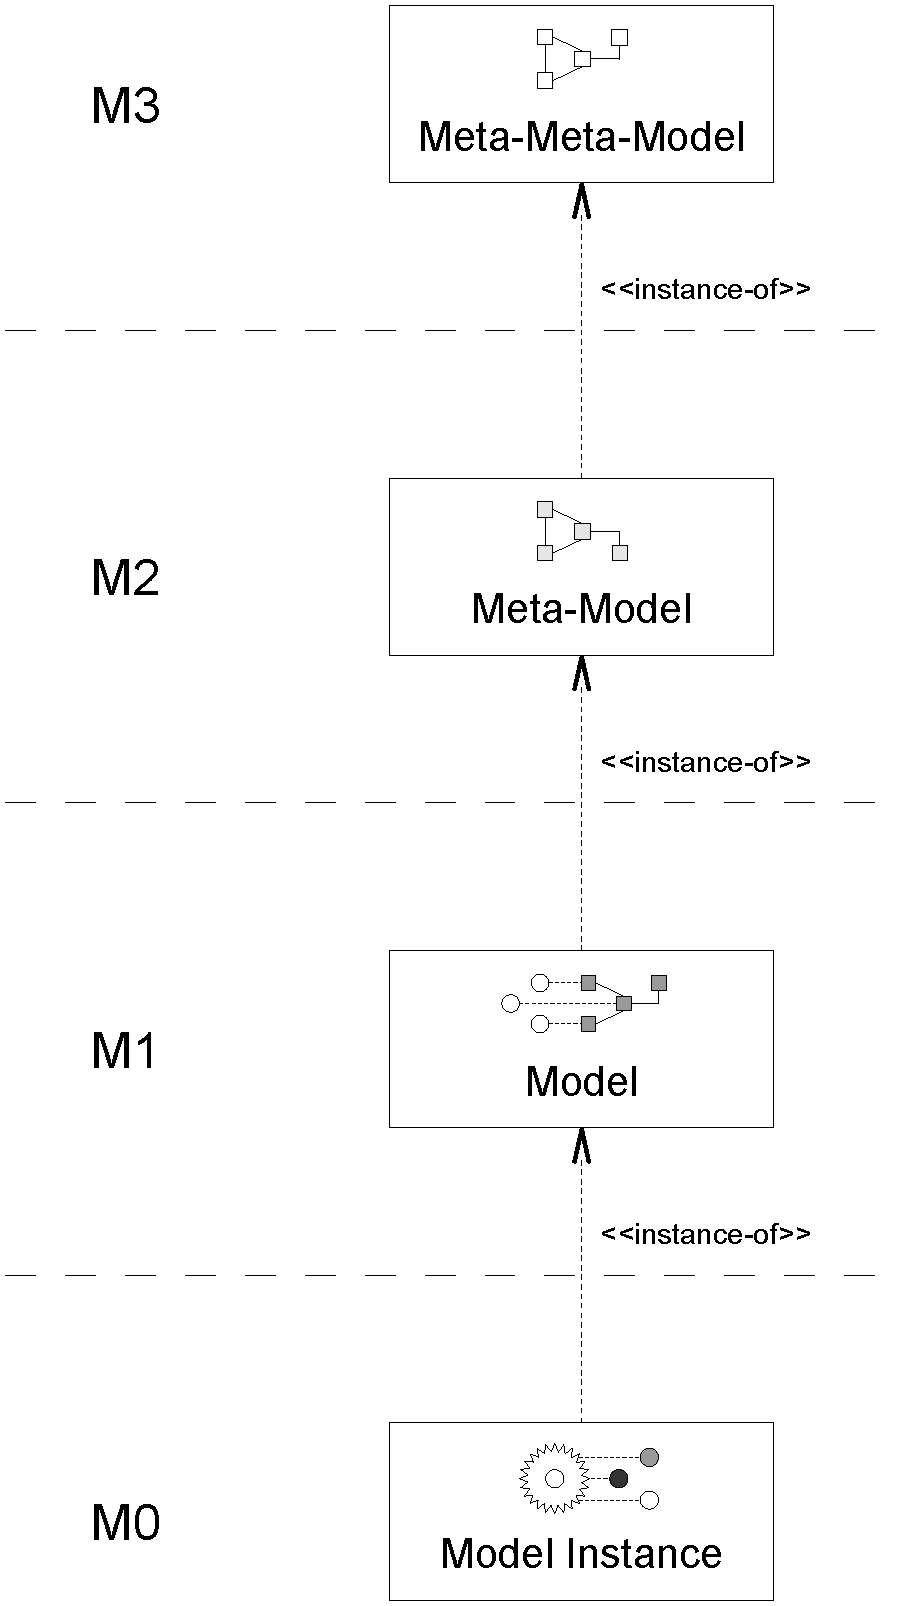
\includegraphics[width=.4\linewidth]{figures/architecture/mofLayers}
	\caption{The MOF Four Layer Metadata Architecture.}
	\label{pic:architecture:mofLayers}

  \vspace{4.5em}
  
	\centering
	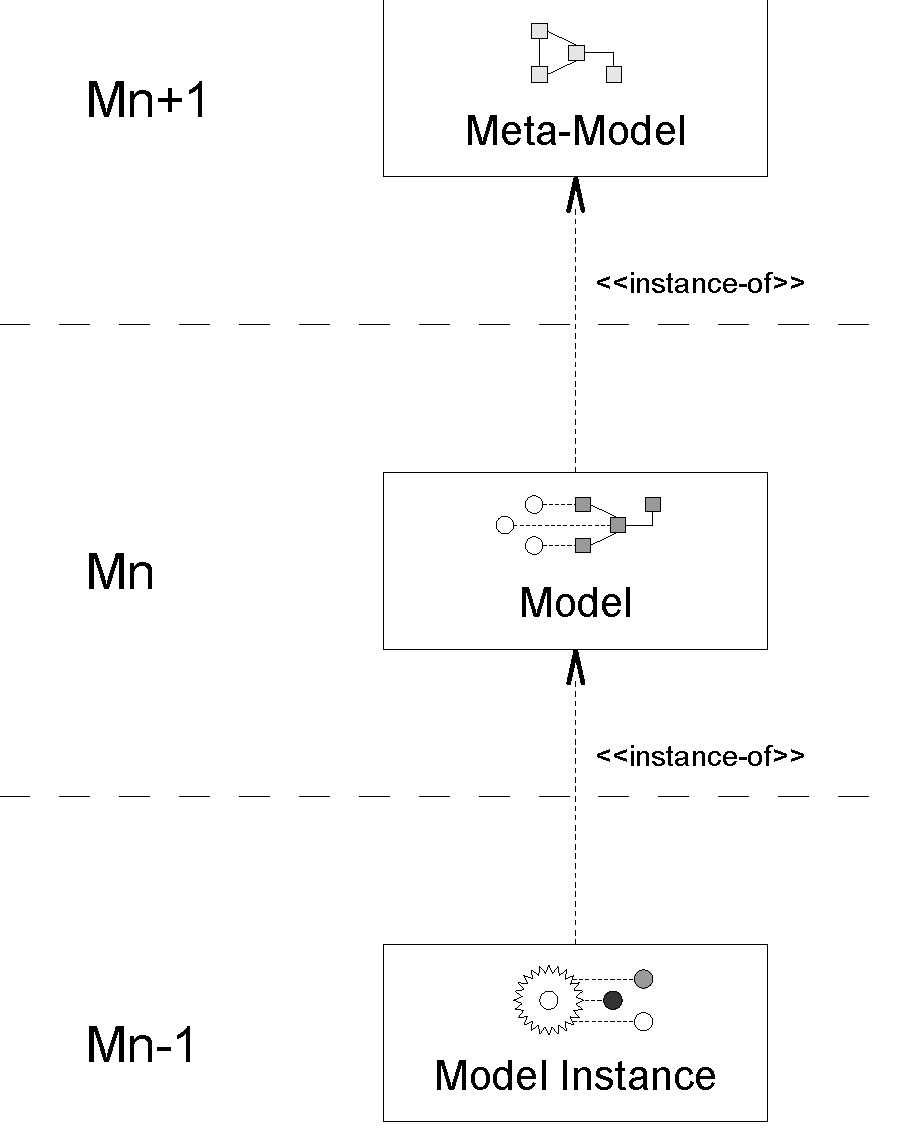
\includegraphics[width=.4\linewidth]{figures/architecture/genericLayers}
	\caption{The Generic Three Layer Metadata Architecture.}
	\label{pic:architecture:genericLayers}

\end{figure}

\acs{OCL} constraints can be defined on both, meta-models and models to verify models or model instances, respectively. E.g., one may use \acs{OCL} to define rules on a meta-model that must be ensured for every model modeled with the meta-model. But, one may use \acs{OCL} to define rules on a model (that must be verified for the model's instances) as well. Thus, the four layer metadata architecture can be generalized to a \keyword{Generic Three Layer Metadata Architecture} in the scope of an \acs{OCL} definition (see Figure \ref{pic:architecture:genericLayers}) \cite{demuth:RGWS09}. On the \keyword{Mn+1 Layer} lies the meta-model that is used to define the model that shall be constrained. On the \keyword{Mn Layer} lies the model that is an instance of the meta-model and can be enriched by the specification of \acs{OCL} constraints. Finally, on the \keyword{Mn-1 Layer} lies the model instance on that the \acs{OCL} constraints shall be verified. Please note, that in the context of such a generic layer architecture, a model
instance can be both a model (like a \acs{UML} class diagram) or a set of objects (like Java run-time objects). 



\section{The Toolkit's Package Architecture}

The package architecture of \acl{DOT4Eclipse} is shown in Figure \ref{pic:architecture:modules}. The architecture is the result of the work of Matthias Br�uer \cite{GB:Braeuer} and can easily be extended. The architecture can be separated into three layers: The \keyword{Back-End}, the \keyword{Core} and the \keyword{Tools Layer}.

\begin{figure}[!b]
	\centering
	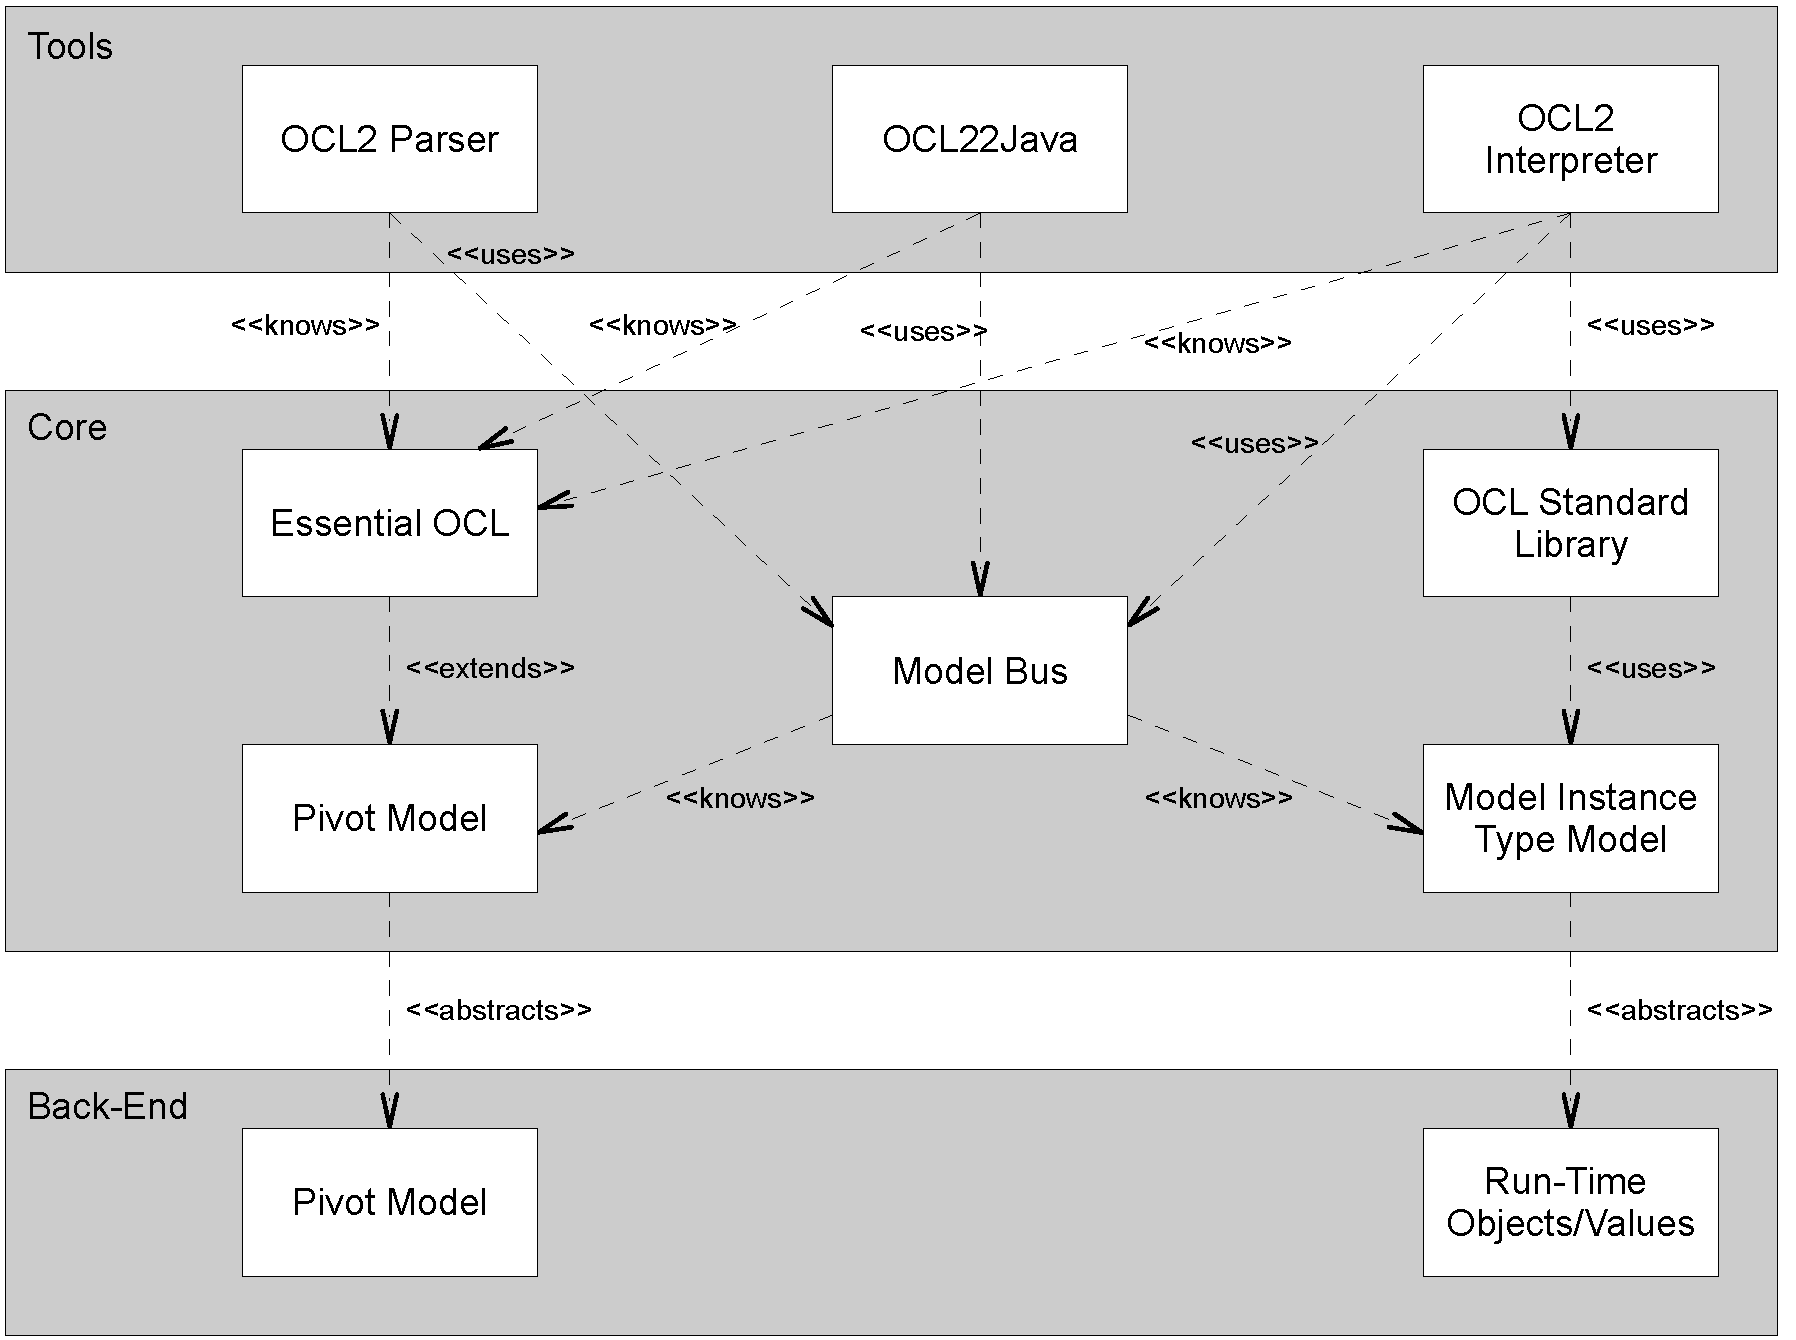
\includegraphics[width=1.0\linewidth]{figures/architecture/modules}
	\caption{The architecture of Dresden OCL2 for Eclipse.}
	\label{pic:architecture:modules}
\end{figure}

The back-end layer contains the meta-model to manage models and run-time objects (or values) that shall be used during interpretation as model instances. Both, meta-models and model instances can easily be exchanged because all other packages of \acl{DOT4Eclipse} do not directly communicate with the meta-model and the run-time objects but use the \keyword{Pivot Model} and the \keyword{Model Instance Type Model} that delegate all requests instead. Important is the fact, that both meta-models and model instances can be exchanged independently. Thus, a Java model instance could be both an instance of a \acs{UML} class diagram and an \acs{EMF} Ecore model.

The second layer is the toolkit's core layer and contains the \keyword{Pivot Model}, \keyword{Essential OCL}, the \keyword{Model Instance Type Model}, the \keyword{\acs{OCL} Standard Library} and the \keyword{Model Bus}. The use of the pivot model and the model instance type model were explained before. The package \keyword{Essential OCL} extends the pivot model and provides the \keyword{Abstract Syntax} to extend loaded models with \acs{OCL} constraints. The \acs{OCL} standard library provides an implementation of all core operations that exist in \acs{OCL} for specific datatypes (e.g., collection iterators like \code{forAll()} or the operation \code{oclIsTypeOf()}). The package \keyword{Model Bus} loads, manages and provides access to models and model instances the user wants to work with and thus, can be considered as the repository of the toolkit.

The third layer contains all tools that are provided with the toolkit. This layer contains the \keyword{\acs{OCL}2 Parser} (which is essential, because the other tools require models that are enriched with already parsed and syntactically and semantically checked constraints), the \keyword{\acs{OCL}2 Interpreter},  and the \keyword{\acs{OCL}22Java Code Generator}. All the tools use the packages of the second layer to access models and model instances and to work on \acs{OCL} constraints. The \acs{OCL} standard library, and also managed model instances are only required by the \acs{OCL}2 interpreter.

\acl{DOT4Eclipse} has been developed as a set of Eclipse/\acs{OSGi} plug-ins. All packages that are located in the core and tools layer represent different Eclipse plug-ins. Additionally, \acl{DOT4Eclipse} contains some plug-ins to provide \acs{GUI} elements such as wizards and examples to run \acl{DOT4Eclipse} with some simple models and \acs{OCL} expressions.



\section{Dresden OCL2 for Eclipse and the Generic Three La\-yer Me\-ta\-da\-ta Architecture}
\label{theory:DOTLayers}

\begin{sidewaysfigure}
	\centering
	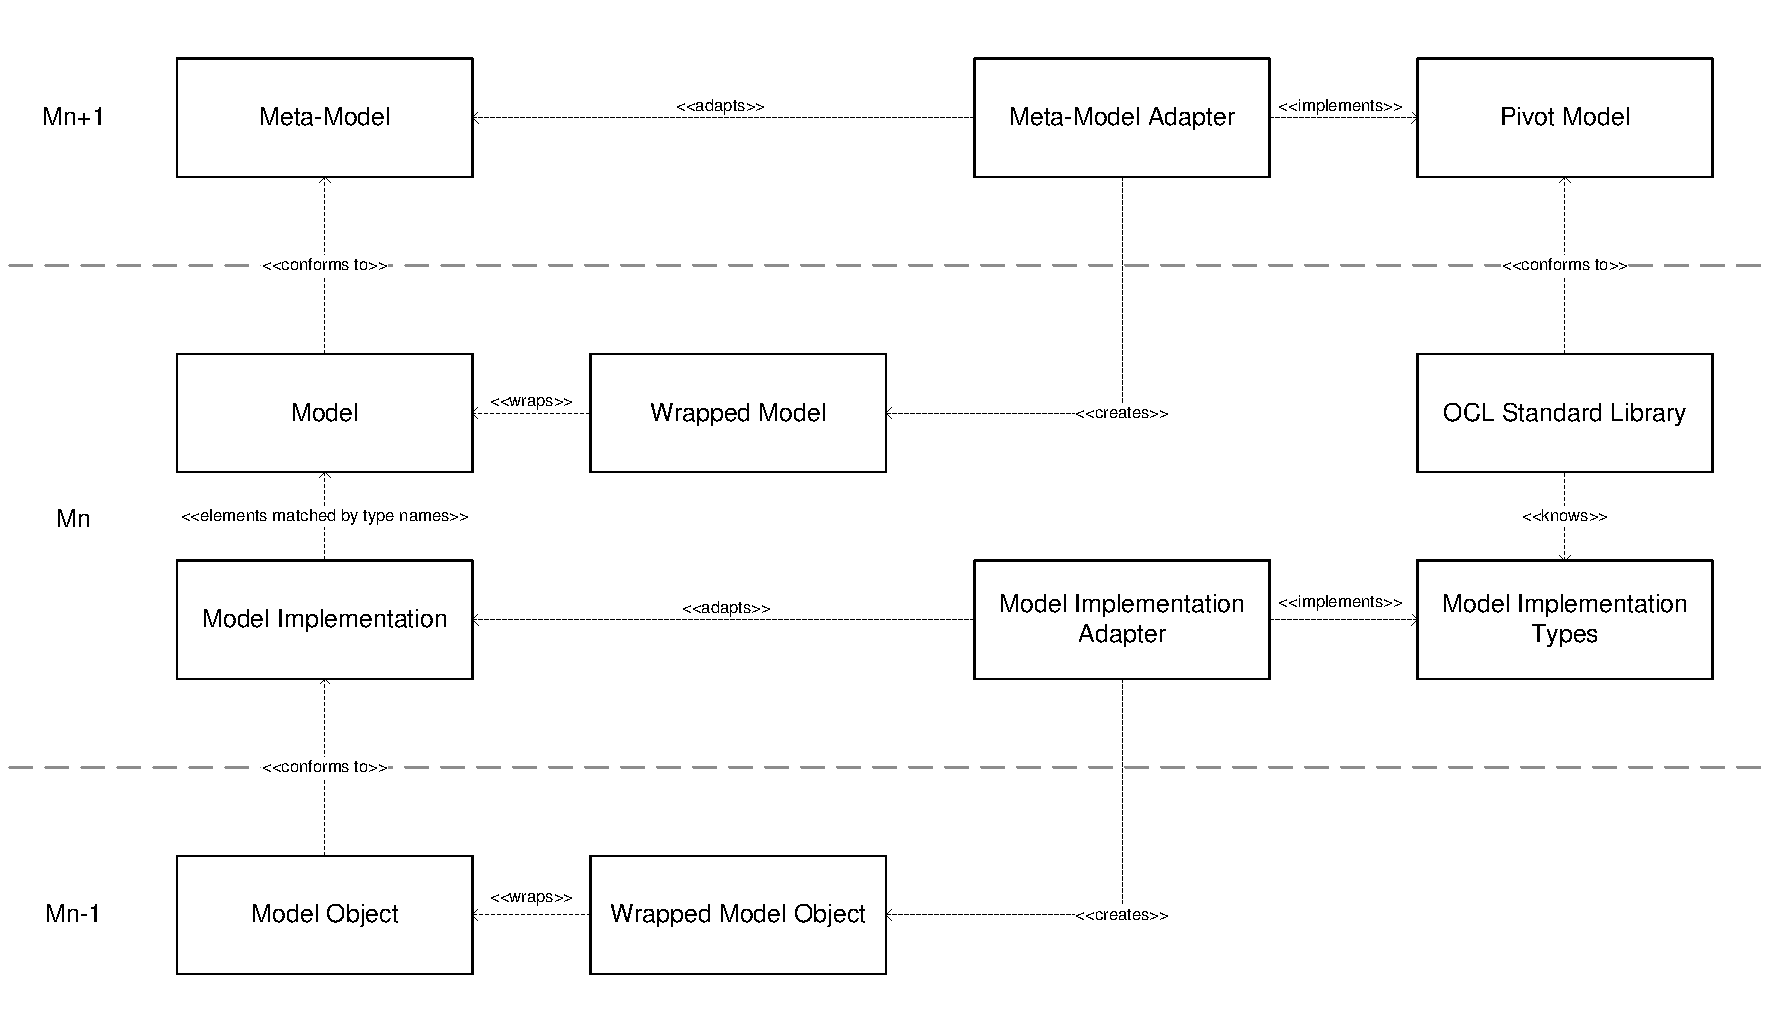
\includegraphics[width=1.0\linewidth]{figures/architecture/modeladaptation}
	\caption{The architecture of Dresden OCL2 for Eclipse in respect to the Generic Three Layer Metadata Architecture.}
	\label{pic:architecture:genericArchitecture}
\end{sidewaysfigure}

Figure \ref{pic:architecture:genericArchitecture} shows the architecture of \acl{DOT4Eclipse} in respect to the Generic Three Layer Metadata Architecture (introduced in Section \ref{architecture:genericLayers}). At the first sight, the architecture seems to be very complex. But do not be afraid! The architecture will now be explained step by step.


\subsection{The Adaptation of Meta-Models, Models and Model Instances}

As you can see, the left part of Figure \ref{pic:architecture:genericArchitecture} shows the Generic Three Layer Metadata Architecture. Meta-models, models and model instances are adapted and loaded into \acl{DOT4Eclipse}. It could be argued that such an adaptation is expensive and costly, but the opposite is the truth. The architecture of \acl{DOT4Eclipse} allows its users to adapt the toolkit to every meta-model and model instance type they want. After the adaptation of a new meta-model or model-instance, they can reuse the rest of the toolkit! Thus, to adapt the \acs{OCL}2 Interpreter to a new type of model instance, only one adaptation is required. The rest comes for free! How to adapt meta-models and model instance types to \acl{DOT4Eclipse} is explained in the Chapters \ref{chapter:pivotModelAdaptation} and \ref{chapter:modelInstanceTypeAdaptation}.


\subsection{How Meta-Models and Models are Adapted}

As already said, the core feature of \acl{DOT4Eclipse} is the \keyword{Pivot Model}. The pivot model is a meta-model that abstracts from all other meta-models. It contains interfaces to define the structural part of a model such as \code{Types}, \code{Namespaces}, \code{Operations} and \code{Properties}. Furthermore, these interfaces provide methods to reason on them (e.g., the interface \code{Namespace} provides a method \code{getNestedNamespaces()} to retrieve all contained \code{Namespaces}).

Every meta-model users want to work with can be adapted to the pivot model. The \keyword{Adapted Meta-Model} must implement the interfaces of the pivot model and must adapt them to its meta-model elements. E.g., adapting the \acs{UML}2 meta-model, the interface \code{Type} from the pivot model must be adapted to the meta-model element \code{UML2Class}. Besides the adaptation of the pivot model, each meta-model must provide a \code{ModelProvider} that provides methods to load model resources of the adapted meta-model and adapts them to its pivot model implementation. The result is a \keyword{Wrapped Model}, \acl{DOT4Eclipse} can work with. Further details about the adaptation of meta-models to the pivot model can be found in Chapter \ref{chapter:pivotModelAdaptation}.


\subsection{How Model Instances are Adapted}

If the \acs{OCL}2 Interpreter shall be used to interpret instances of a loaded model, a second adaptation is required, an adaptation to the \keyword{Model Instance Type Model}. The model instance type model can be considered as similar to the pivot model, but the purpose is different. If \acs{OCL} constraints shall be interpreted on run-time objects or values, operations and properties of these run-times values must be accessible. E.g., if a constraint like \code{context Person inv: age >= 0} shall be interpreted, the property \code{age} of a run-time object of the class \code{Person} must be accessed. The \acs{OCL}2 interpreter does not accesses this property directly, but delegates the request to a model instance type adaptation to let the model instance type become exchangeable\footnote{To be honest, the interpreter does not delegate the access directly but uses the \acs{OCL} standard library instead which delegates the request to the model instance. But this is a technical detail and not important in this context.}. Thus, \acl{DOT4Eclipse} contains a second model the \keyword{Model Implementation Type Model} that can be considered as an abstraction of all model instance types. The model instance type model defines a set of interfaces to describe the elements of a model instance (e.g., \code{IModelInstancePrimitiveType} and \code{IModelInstanceObject}). These interfaces provide operations to reflect on the model instance objects (e.g., the operation \code{IModelInstanceType.invokeOperation()} or the operation \code{IModelInstanceElement.isTypeOf()}). The reflection mechanism can be considered as similar to the mechanism provided by Java in the package \code{java.lang.reflect}.

Each model instance type users want to work with must be adapted to the model instance type model. Besides an adaptation of the interfaces, also a \code{ModelInstanceProvider} must be implemented that is responsible to adapt model instance objects to the implemented interfaces. Due to the fact of this second adaptation, \acl{DOT4Eclipse} is able to use the same \acs{OCL}2 Interpreter for different types of model instances! More details about the adaptation of model instances to \acl{DOT4Eclipse} are available in Chapter \ref{chapter:modelInstanceTypeAdaptation}.


\subsection{Coupling between Models and their Instances}

As mentioned above, different types of models can be connected with different types of instances. E.g., a \acs{UML} class diagram could be implemented by a set of Java Classes (and their objects) or by an \acs{XML} document. To maintain this loose coupling, meta-models and model implementation types do not know each other. If a model instance is imported into \acl{DOT4Eclipse}, a model (and thus also a meta-model) has to be selected, to that the instance belongs to. The objects of the instance are matched to the types of the selected model by the name of their types. E.g., a Java instance's objects are matched by associating their classes' names to the names of the types of the selected model.


\subsection{Essential OCL and OCL Constraints}

To enrich models loaded into \acl{DOT4Eclipse} with \acs{OCL} constraints, a meta-model for \acs{OCL} constraints is required (also called the \keyword{Abstract Syntax}). This meta-model contains elements like \code{OperationCallExpressions} or \code{StringLiterals} to describe the different tokens of \acs{OCL} constraints and to enrich loaded models with parsed \acs{OCL} constraints. \keyword{Essential \acs{OCL}} is this \acs{OCL} meta-model that is used by the \acs{OCL}2 Parser to build the model representation of parsed \acs{OCL} constraints. Essential \acs{OCL} extends the pivot model, because \acs{OCL} constraints can also contain \code{Types}, \code{Operations} and \code{Properties} defined in the model.


\subsection{The OCL Standard Library}

The \keyword{\acs{OCL} Standard Library} is required when \acs{OCL} constraints shall be interpreted. The \acs{OCL} standard library is the implementation of all operations that are defined in the \acs{OCL} standard and are available for all types in \acs{OCL} or for different kinds of types (e.g., the operations \code{String.concat()} or \code{OclAny.oclIsUndefined()}. The \acs{OCL} standard library is invoked by the \acs{OCL}2 Interpreter at any time, the interpreter wants to interpret the value of an \code{OperationCallExpression} or a \code{PropertyCallExpression}. The \acs{OCL} standard library either computes the result itself or delegates the request to an adapted model instance (via the \keyword{Model Implementation Type Model}'s interfaces) if a model-specific operation or property shall be accessed.



\section{Summary}

This Chapter introduced into the architecture and package structure of \acl{DOT4Eclipse}. The \keyword{Pivot Model} and the \keyword{Model Implementation Type Model} have been explained shortly. Also the relationships between the pivot model, \keyword{Essential \acs{OCL}} and the \keyword{\acs{OCL} Standard Library} have been presented. One may argue that the architecture seems to be complex and complicate. Nevertheless, it should be remembered that \acl{DOT4Eclipse} was designed as generic as possible. Thus, \acl{DOT4Eclipse} can be adapted to various different kinds of meta-models and model instances without changing the \acs{OCL}2 Parser nor the \acs{OCL}2 Interpreter!